\newpage
\section{Results}\label{ch:results}
\subsection{Reporting Conventions}
All numbers are means over ten seeds unless stated otherwise. Tables report test Macro-F1 under the strict protocol P3 unless a different protocol is named. The test set has 317 rows. M0 always predicts the training majority class; M0r guesses uniformly at random and is the appropriate floor for Macro-F1. Every value below is taken from the executed ten-seed run; no hyper-parameter was changed after the pilot run (pilot outputs were not saved, so this cannot be independently verified); M0r and M6 were added after the pilot.

\subsection{Overall Comparison Under the Strict Protocol}\label{sec:overall}
\begin{table}[H]
\centering
\begin{tabular}{llcccc}
\toprule
Model & Inputs & Macro-F1 & Accuracy & Balanced acc.\\
\midrule
M0 & majority class & 0.207 $\pm$ 0.000 & 0.451 & 0.333\\
M0r & uniform random guess & 0.333 $\pm$ 0.020 & 0.339 & 0.341\\
M1 & price window & \textbf{0.466} $\pm$ 0.036 & 0.530 & 0.476\\
M2 & price + FinBERT embedding & 0.416 $\pm$ 0.023 & 0.493 & 0.448\\
M3 & price + embedding + regime & 0.433 $\pm$ 0.025 & 0.491 & 0.454\\
M4 & embedding only & 0.382 $\pm$ 0.037 & 0.402 & 0.394\\
M5 & regime only & 0.354 $\pm$ 0.019 & 0.493 & 0.415\\
M6 & price + sentiment (3 scores) & \textbf{0.482} $\pm$ 0.038 & 0.531 & 0.498\\
\bottomrule
\end{tabular}
\caption[Test performance under the strict protocol P3]{Test performance under the strict protocol P3 (Macro-F1 mean $\pm$ s.d.\ over 10 seeds). M1 and M6 are not reliably different (Table~\ref{tab:diffs}).}\label{tab:main}
\end{table}
All learned models exceed the random-guess floor. The price-only model is competitive with every richer model, the news-only model reaches 0.382, and the regime-only model is close to the floor in Macro-F1 although its accuracy (0.493) is similar to that of the richer models, which shows why accuracy alone is a poor guide on this data.

\begin{table}[H]
\centering
\begin{tabular}{lcccc}
\toprule
Model & Train Macro-F1 & Valid Macro-F1 & Test Macro-F1 & Train $-$ Test\\
\midrule
M0 & 0.232 & 0.249 & 0.207 & 0.025\\
M0r & 0.315 & 0.291 & 0.333 & $-$0.018\\
M1 & 0.477 & 0.464 & 0.466 & 0.011\\
M2 & 0.554 & 0.452 & 0.416 & 0.138\\
M3 & 0.569 & 0.461 & 0.433 & 0.136\\
M4 & 0.701 & 0.378 & 0.382 & 0.319\\
M5 & 0.360 & 0.390 & 0.354 & 0.006\\
M6 & 0.486 & 0.456 & 0.482 & 0.004\\
\bottomrule
\end{tabular}
\caption[Train, validation and test Macro-F1 under P3 (table)]{Macro-F1 on training, validation and test rows under P3 (mean over 10 seeds). Large train--test gaps for the models using the 768-dimensional embedding (M2, M3, M4) indicate overfitting.}\label{tab:overfit}
\end{table}
Table~\ref{tab:overfit} shows that the price-only model has almost no train--test gap (0.477 versus 0.466), whereas adding the 768-dimensional embedding raises training Macro-F1 to 0.554 and lowers test Macro-F1 to 0.416. The news-only model fits training rows well (0.701) but generalises poorly (0.382). Figure~\ref{fig:tvt} shows the same numbers: for M2, M3 and M4 the training bar sits well above the validation and test bars, whereas for M1 and M6 the three bars are close.
\begin{figure}[H]\centering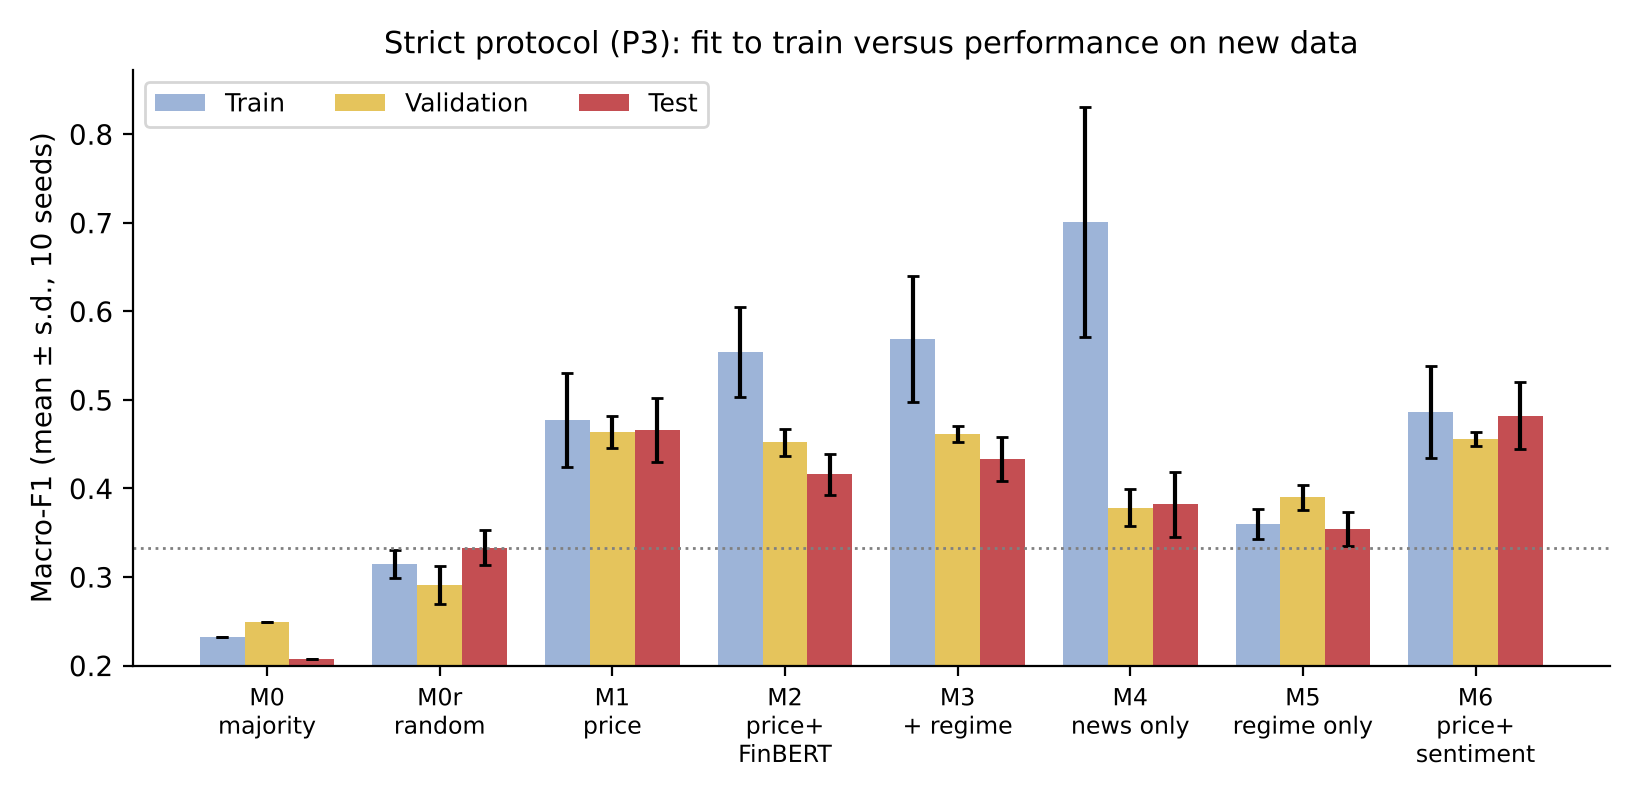
\includegraphics[width=\textwidth]{fig_train_valid_test.png}\caption[Train, validation and test Macro-F1 under P3 (figure)]{Macro-F1 on training, validation and test rows under P3 (mean $\pm$ s.d.\ over ten seeds; dotted line: random-guess level 0.333). Same values as Table~\ref{tab:overfit}.}\label{fig:tvt}\end{figure}

\subsection{Effect of the Evaluation Protocol (RQ1)}\label{sec:protocol-results}
\begin{table}[H]
\centering
\begin{tabular}{lccc}
\toprule
Model & P1 random, fit all & P2 chronological, fit all & P3 strict\\
\midrule
M0 & 0.228 & 0.207 & 0.207\\
M0r & 0.315 & 0.333 & 0.333\\
M1 price & 0.438 & 0.460 & 0.466\\
M2 price + embedding & 0.423 & 0.428 & 0.416\\
M3 price + emb.\ + regime & 0.421 & 0.441 & 0.433\\
M4 embedding only & 0.363 & 0.369 & 0.382\\
M5 regime only & 0.400 & 0.382 & 0.354\\
M6 price + sentiment & 0.431 & 0.448 & 0.482\\
\bottomrule
\end{tabular}
\caption{Test Macro-F1 by protocol (mean over 10 seeds).}
\end{table}
\begin{table}[H]
\centering
\begin{tabular}{lcc}
\toprule
Model & P1 $-$ P3 & P2 $-$ P3\\
\midrule
M1 & $-0.028$ [$-0.055$, 0.001] & $-0.005$ [$-0.034$, 0.023]\\
M2 & $+0.006$ [$-0.010$, 0.022] & $+0.012$ [$-0.008$, 0.031]\\
M3 & $-0.012$ [$-0.030$, 0.008] & $+0.008$ [$-0.010$, 0.028]\\
M4 & $-0.019$ [$-0.040$, 0.004] & $-0.013$ [$-0.043$, 0.018]\\
M5 & \textbf{$+0.046$ [0.029, 0.063]} & \textbf{$+0.028$ [0.007, 0.048]}\\
M6 & \textbf{$-0.051$ [$-0.079$, $-0.019$]} & $-0.034$ [$-0.071$, 0.005]\\
\bottomrule
\end{tabular}
\caption[Protocol gaps (looser protocol minus P3) with 95\% intervals]{Optimistic performance gap (looser protocol minus P3) with 95\% bootstrap intervals over seeds. Positive values mean the looser protocol scores higher. Intervals resample the ten seeds of each protocol independently; they exclude test-row uncertainty, and P1 also changes the test sample.}\label{tab:gaps}
\end{table}
\begin{figure}[H]\centering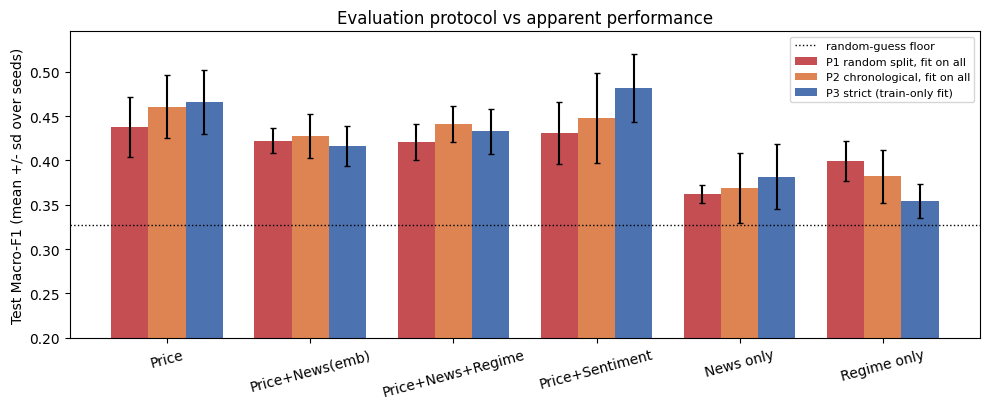
\includegraphics[width=\textwidth]{fig_protocol_audit.png}\caption[Test Macro-F1 under the three evaluation protocols]{Test Macro-F1 under the three evaluation protocols (mean over ten seeds, error bars $\pm1$ s.d.; dotted line: mean random-guess score, about 0.33). The protocol gaps are in Table~\ref{tab:gaps}.}\end{figure}
Figure~\ref{fig:seeds} plots every one of the 240 evaluations behind these bars. For the trained models the standard deviation over the ten seeds is between 0.010 and 0.051 depending on model and protocol (0.019 to 0.038 under P3, Table~\ref{tab:main}), which is as large as many of the differences between models and protocols; this is why intervals, rather than point differences, are used throughout. The majority-class baseline M0 has almost no spread under P2 and P3 because it is deterministic, and the regime-only model M5 repeats a few values, as expected for an input that takes only three distinct values.
\begin{figure}[H]\centering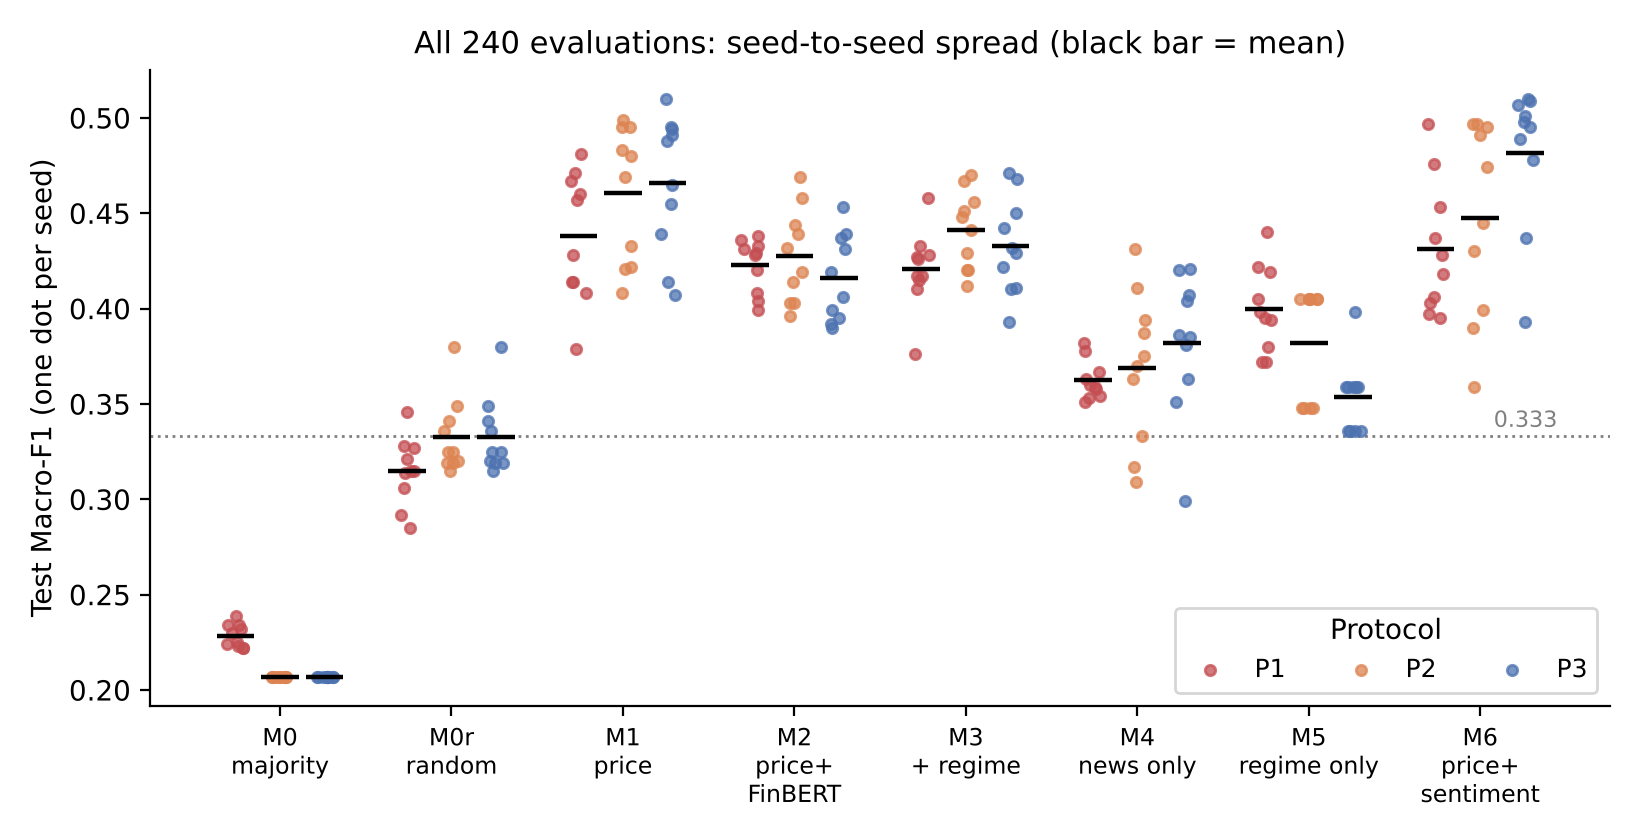
\includegraphics[width=\textwidth]{fig_seed_scatter.png}\caption[Test Macro-F1 of all 240 model--protocol--seed evaluations]{Test Macro-F1 of each of the 240 model--protocol--seed evaluations (one dot per seed; black bar: mean over seeds; dotted line: 0.333).}\label{fig:seeds}\end{figure}

For the models that use lagged prices and/or news (M1--M4) the looser protocols did \emph{not} score reliably higher than the strict one; all eight intervals for M1--M4 include zero. The exception is the regime-only model M5, which scores higher under both looser protocols (+0.046 and +0.028). Two mechanisms could contribute and were not separated here: under P1 a random split places near neighbours of each test day in the training set, and under P1 and P2 fitting the clusters on all data lets test-period structure shape the regime labels. P2$-$P3 shares the test rows and is the cleaner contrast (+0.028, interval near zero). For M6 the strict protocol scored \emph{higher} than the random split. This reversal reinforces that the protocol gaps are model-dependent; because P1 changes the test sample across seeds, the observed gap also reflects sample composition and run-to-run variability, not leakage alone. Hypothesis H1 is therefore \textbf{not supported in general}, and only weakly and exploratorily suggested for the model that relies solely on a slowly varying state.

\subsection{Value of News and Regime Information (RQ2)}\label{sec:regime-results}
\begin{table}[H]
\centering
\small
\begin{tabular}{lrccccc}
\toprule
Group & $n$ & Random & M1 & M2 & M3 & M6\\
 & & floor & price & +emb. & +emb.+reg. & +sent.\\
\midrule
All test & 317 & 0.333 & 0.466 & 0.416 & 0.433 & 0.482\\
Low-vol & 125 & 0.329 & 0.409 & 0.386 & 0.407 & 0.415\\
Mid-vol & 113 & 0.322 & 0.410 & 0.341 & 0.361 & 0.464\\
High-vol & 79 & 0.323 & 0.357 & 0.363 & 0.319 & 0.378\\
Stress window & 50 & 0.316 & 0.473 & 0.448 & 0.450 & 0.471\\
Outside stress & 267 & 0.334 & 0.451 & 0.391 & 0.416 & 0.467\\
\bottomrule
\end{tabular}
\caption[Test Macro-F1 by group under P3]{Test Macro-F1 by group under P3 (mean over ten seeds of the per-seed Macro-F1 on the group's rows). Group sizes are small, so group-level values are noisy.}\label{tab:levels}
\end{table}
\begin{table}[H]
\centering
\small
\begin{tabular}{lrccc}
\toprule
Group & $n$ & M2 $-$ M1 & M6 $-$ M1 & M3 $-$ M2\\
 & & (embedding) & (sentiment) & (regime input)\\
\midrule
All test & 317 & \textbf{$-0.050$ [$-0.087$, $-0.012$]} & $+0.016$ [$-0.017$, 0.049] & $+0.017$ [$-0.002$, 0.038]\\
Low-vol & 125 & $-0.023$ [$-0.079$, 0.031] & $+0.006$ [$-0.041$, 0.058] & $+0.021$ [$-0.002$, 0.043]\\
Mid-vol & 113 & $-0.069$ [$-0.147$, 0.003] & \textbf{$+0.054$ [0.004, 0.107]} & $+0.021$ [$-0.011$, 0.051]\\
High-vol & 79 & $+0.005$ [$-0.062$, 0.074] & $+0.020$ [$-0.041$, 0.081] & $-0.043$ [$-0.101$, 0.011]\\
Stress window & 50 & $-0.024$ [$-0.115$, 0.056] & $-0.001$ [$-0.079$, 0.072] & $+0.002$ [$-0.044$, 0.046]\\
Outside stress & 267 & \textbf{$-0.060$ [$-0.097$, $-0.017$]} & $+0.016$ [$-0.021$, 0.050] & \textbf{$+0.024$ [0.002, 0.047]}\\
\bottomrule
\end{tabular}
\caption[Differences in Macro-F1 between models, by group, with 95\% intervals]{Differences in Macro-F1 (second minus first model) with 95\% bootstrap intervals from resampling test rows. Bold: interval excludes zero. For news and regime together versus price only, M3 $-$ M1 is $-0.033$ [$-0.069$, 0.001] overall. Rows are resampled as if independent; temporal dependence is ignored, so intervals are probably too narrow.}\label{tab:diffs}
\end{table}
\begin{figure}[H]\centering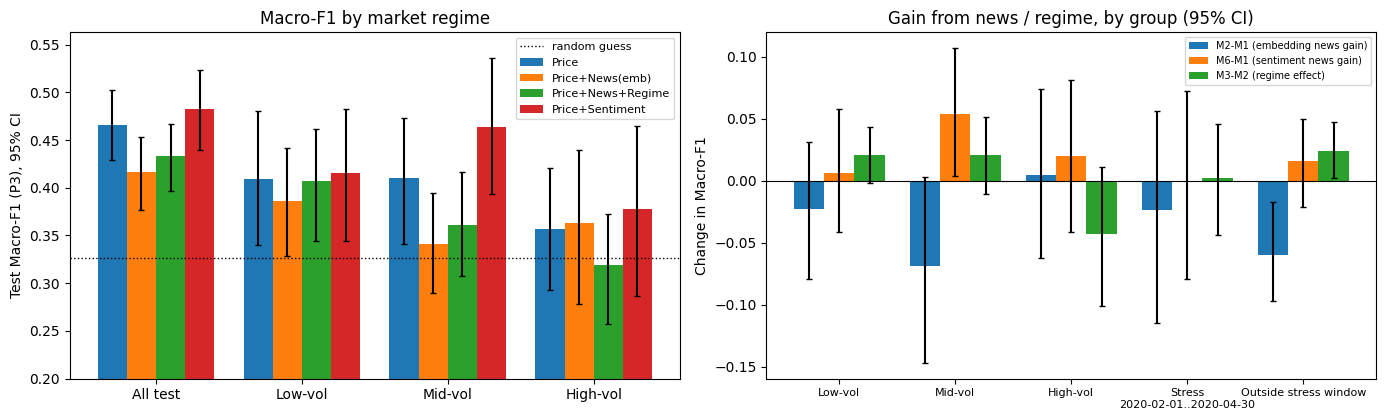
\includegraphics[width=\textwidth]{fig_regime_news_value.png}\caption[Macro-F1 and model differences by regime and stress window]{Test Macro-F1 (left) and model differences (right) by regime and stress window under P3, with 95\% row-bootstrap intervals; error bars are the intervals of Tables~\ref{tab:levels} and~\ref{tab:diffs}.}\end{figure}
Four findings follow.
\begin{enumerate}
\item \textbf{The FinBERT embedding hurts.} Adding it to the price model reduces Macro-F1 by 0.050 with an interval excluding zero; outside the stress window the reduction is 0.060.
\item \textbf{A low-capacity news input is about neutral.} Three sentiment scores give $+0.016$ overall with an interval including zero. The only interval excluding zero (Mid-vol, $+0.054$) is one of 24 comparisons and is treated as a hypothesis.
\item \textbf{The regime input adds little.} Adding the regime id to the price-plus-embedding model changes Macro-F1 by $+0.017$ (interval includes zero); the best news-plus-regime model (M3) does not beat price only. Outside the stress window the regime input gives $+0.024$ [0.002, 0.047], one of four intervals excluding zero (with M2$-$M1 overall and outside stress, and M6$-$M1 in Mid-vol); all four are treated as exploratory.
\item \textbf{No reliable extra news value detected in the stress window.} In 1 February--30 April 2020 no model with news information differs reliably from price only. With only 50 rows the intervals are wide (about $\pm0.05$ to $\pm0.09$), so moderate effects cannot be excluded.
\end{enumerate}

\subsection{The Stress Window}\label{sec:stress}
Within the stress window the price-only model reaches 0.473, the random floor 0.316, and the embedding and regime models 0.448 and 0.450. None of the news-related differences is reliably non-zero (Table~\ref{tab:diffs}). Mean FinBERT sentiment in March 2020 is $-0.319$ against $-0.176$ for the remainder of the test set, so the headlines do register the shock, but this did not translate into a measurable gain in next-day classification.

\subsection{Diagnostic: What the Models Predict}
Table~\ref{tab:classdiag} shows predicted class shares and per-class F1 for the price-only and sentiment models.
\begin{table}[H]
\centering
\begin{tabular}{lccc}
\toprule
 & Fall & Neutral & Rise\\
\midrule
True test share & 0.230 & 0.451 & 0.319\\
M1 predicted share & 0.191 & 0.545 & 0.263\\
M2 predicted share & 0.303 & 0.581 & 0.116\\
M3 predicted share & 0.302 & 0.525 & 0.173\\
M6 predicted share & 0.322 & 0.502 & 0.176\\
M1 per-class F1 & 0.291 & 0.687 & 0.420\\
M6 per-class F1 & 0.397 & 0.690 & 0.358\\
\bottomrule
\end{tabular}
\caption{Predicted shares and per-class F1 on the P3 test set (10 seeds).}\label{tab:classdiag}
\end{table}
The Neutral-class F1 is almost identical for M1 and M6 (0.687 and 0.690). The sentiment model trades Rise for Fall (Fall F1 $0.291\to0.397$, Rise F1 $0.420\to0.358$) and predicts Fall on 32\% of days versus 19\% for the price-only model (true share 23\%). This is consistent with the small and unreliable overall change: the news input shifts the balance between the two directional classes but adds no clear skill.

Figure~\ref{fig:shares} shows the predicted shares of Table~\ref{tab:classdiag} against the true shares. All four models predict Neutral more often than its true share (0.451), and the models that use news predict Rise for only 12--18\% of rows against a true share of 32\%, so a large part of the differences in Macro-F1 between models reflects how the predictions are distributed across classes.
\begin{figure}[H]\centering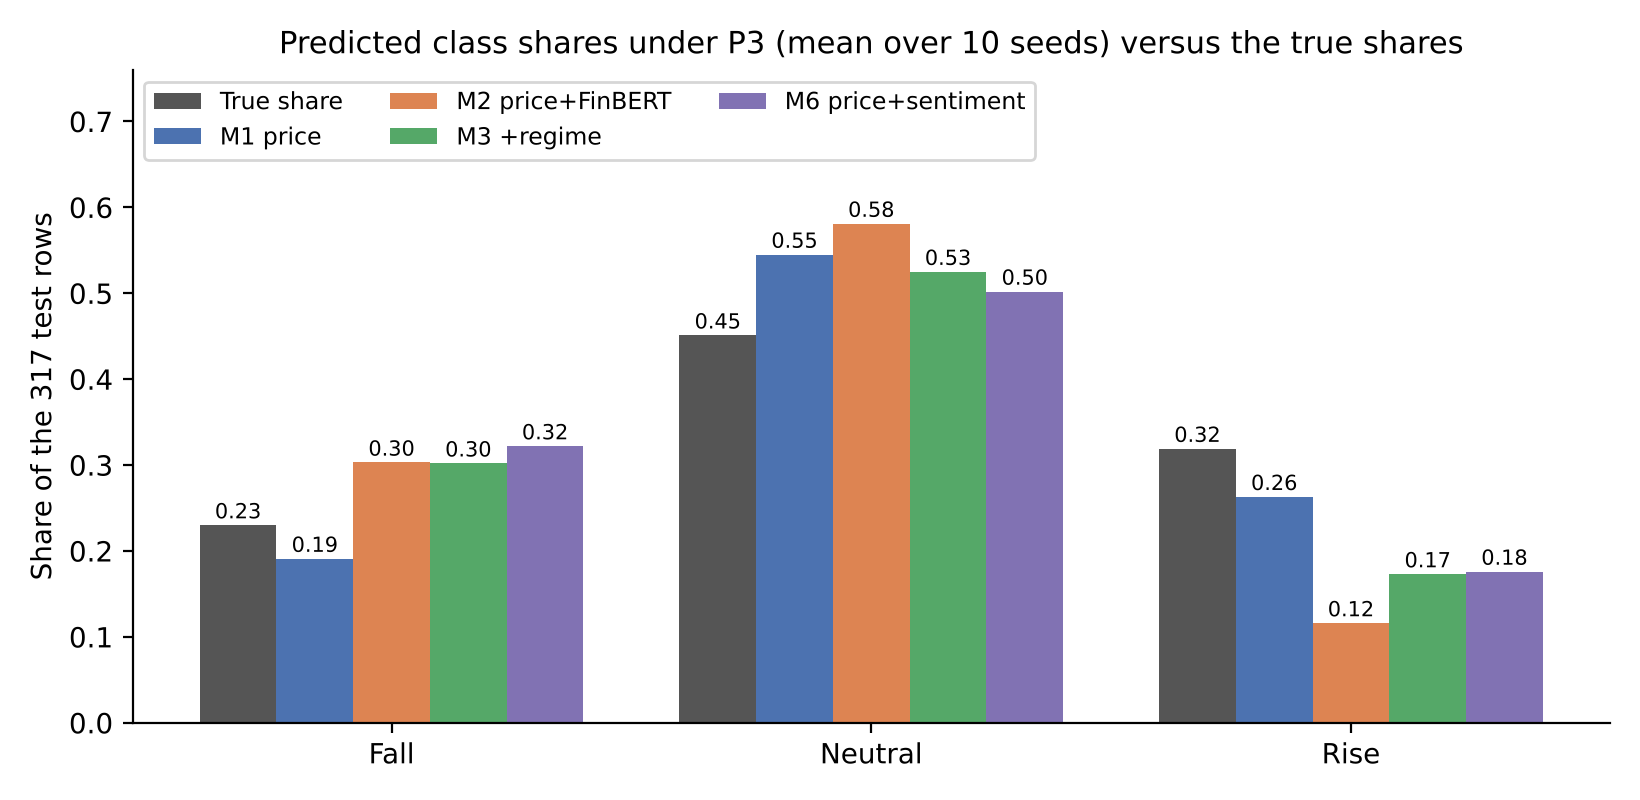
\includegraphics[width=\textwidth]{fig_class_shares.png}\caption[Predicted and true class shares on the P3 test set]{Predicted class shares on the P3 test set (mean over ten seeds) for the price-only, price-plus-embedding, price-plus-embedding-plus-regime and price-plus-sentiment models, against the true shares.}\label{fig:shares}\end{figure}

\subsection{Summary of Hypotheses}
\begin{table}[H]
\centering
\begin{tabular}{p{5.2cm}p{9.3cm}}
\toprule
Hypothesis & Outcome\\
\midrule
H1: looser protocols overstate performance & Not supported in general; weak, exploratory evidence for the regime-only model (M5), with sample composition not separated from leakage.\\
H2: the value of news differs across regimes & Not supported for embeddings (no gain in any regime). For sentiment a gain appears only in Mid-vol and is not robust; insufficient evidence of regime dependence.\\
H3: an explicit regime input improves the multimodal model & Not supported ($+0.017$, interval includes zero; M3 does not beat M1). One interval outside the stress window ($+0.024$) excludes zero and is exploratory.\\
\bottomrule
\end{tabular}
\caption{Outcome of the hypotheses.}
\end{table}
